\documentclass[a4paper, 12pt]{article}
\usepackage[T2A]{fontenc}
\usepackage[utf8]{inputenc}
\usepackage[english,russian]{babel}
\usepackage{amsmath, amsfonts, amssymb, amsthm, mathtools, misccorr, indentfirst, multirow}
\usepackage{wrapfig}
\usepackage{graphicx}
\usepackage{subfig}
\usepackage{adjustbox}
\usepackage{pgfplots}

\usepackage{geometry}
\geometry{top=20mm}
\geometry{bottom=20mm}
\geometry{left=20mm}
\geometry{right=20mm}



\begin{document}
	\begin{titlepage}
	\begin{center}
		\large{МИНИСТЕРСТВО ОБРАЗОВАНИЯ И НАУКИ\\РОССИЙСКОЙ ФЕДЕРАЦИИ}
		
		Федеральное агентство по образованию
		\vspace{0.5cm}
		
		\large{МОСКВОСКИЙ ФИЗИКО-ТЕХНИЧЕСКИЙ ИНСТИТУТ\\(ГОСУДАРСТВЕННЫЙ УНИВЕРСИТЕТ)}
		\vspace{0.5cm}
		
		Кафедра вакуумной электроники
		\vfill
		
		{\LARGE Термоэлектронный диод}
		\bigskip
		
		Лабораторная работа\\
		по курсу: Вакуумная электроника 
	\end{center}
	\vfill
	
	\hfill\begin{minipage}{0.4\textwidth}
		Работу выполнил\\
		студент 654 группы\\
		Нехаев Александр
	\end{minipage}
	\vfill
	
	\begin{center}
		Долгопрудный\\2018 г.
	\end{center}
	\end{titlepage}
	\tableofcontents
	\newpage
	\section{Цели и задачи исследования}
	\begin{enumerate}
		\item Практическое изучение явления термоэлектронной эмиссии и процессов токопрохождения в вакууме;
		\item Изготовление вакуумного диода;
		\item Исследование некоторых характеристик диода;
		\item Проверка справедливости законов Ричардсона-Дешмана и Чайлда-Ленгмюра.
	\end{enumerate}
	\section{Схема установки}
	\begin{figure}[h]
		\centering
		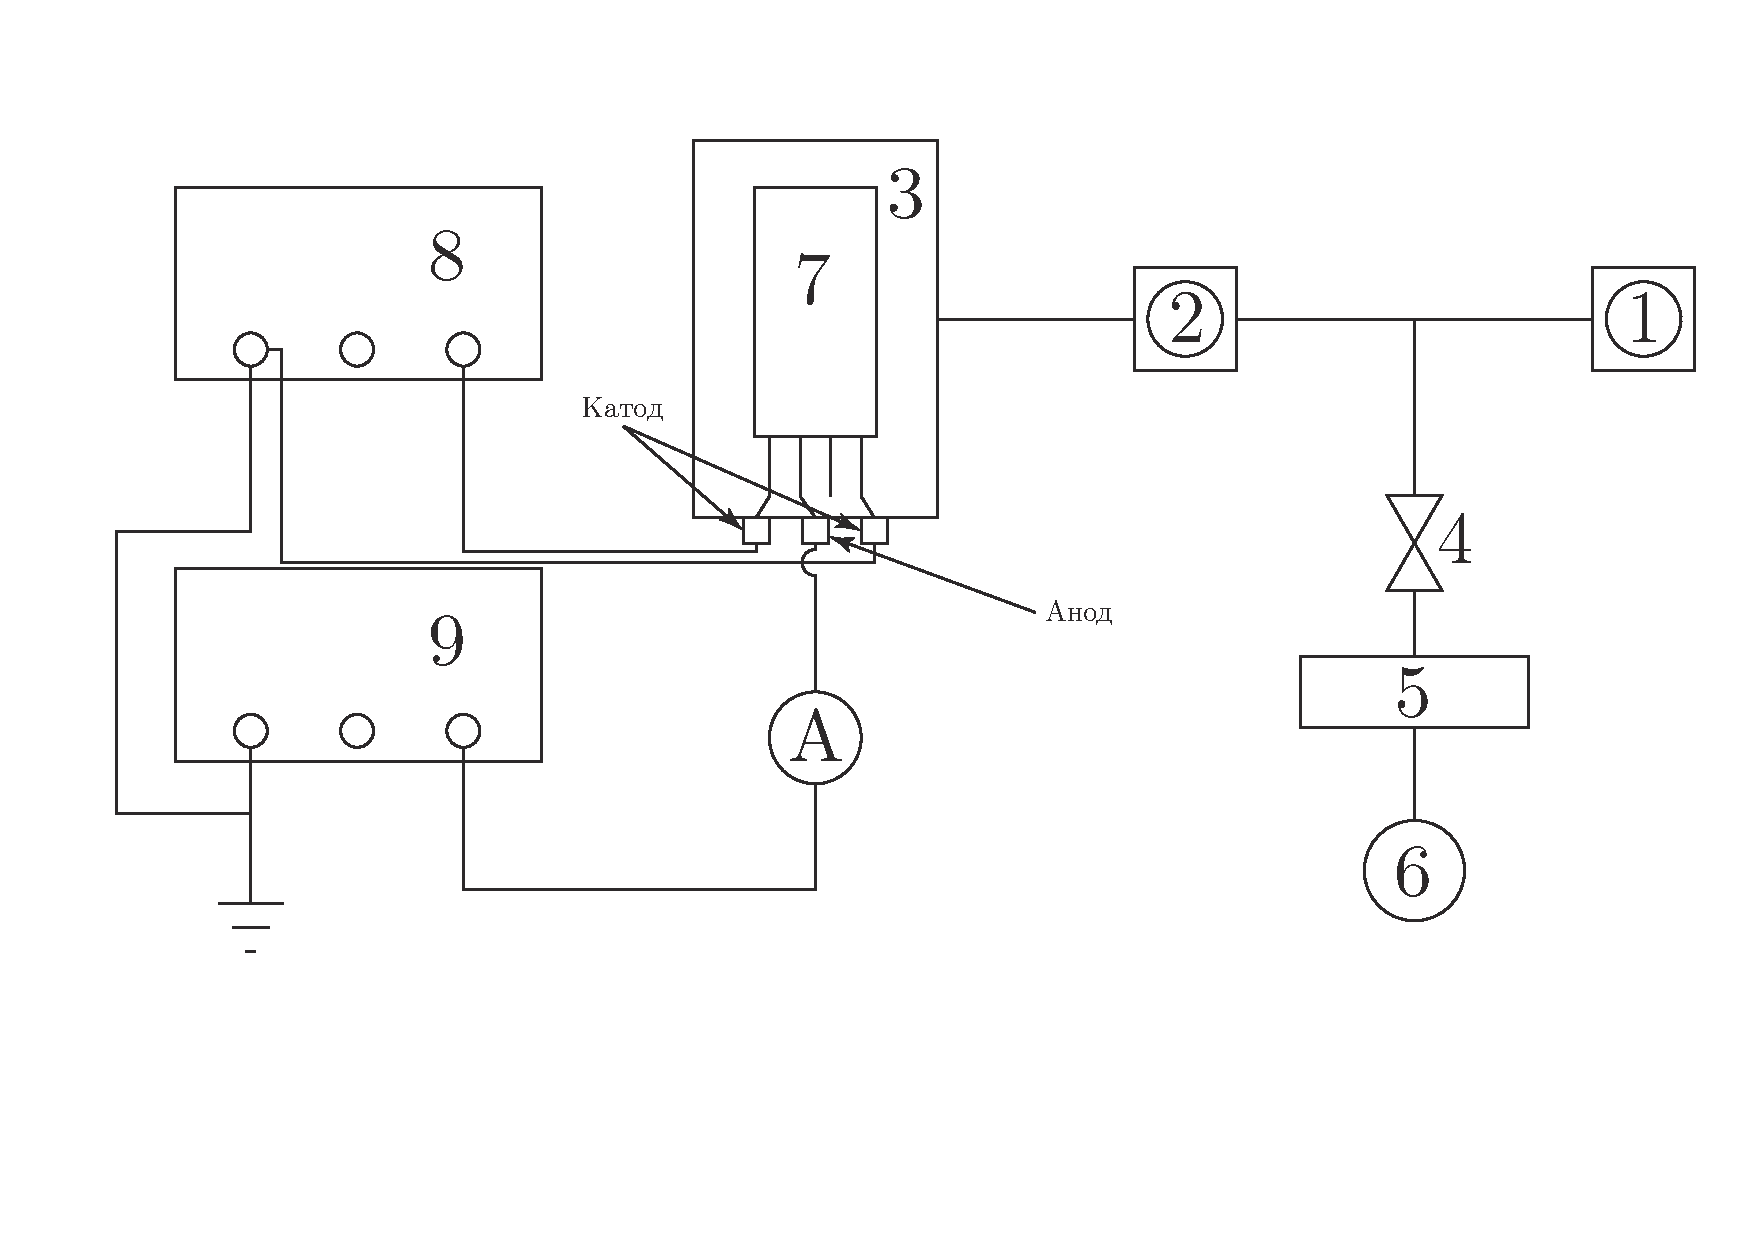
\includegraphics[scale=0.4]{scheme.pdf}
		\caption{Схема установки}
		\label{fig:schematic}
	\end{figure}
	\begin{enumerate}
		\item Форвакуумный насос
		\item Турбомолекулярный насос
		\item Вакуумная камера
		\item Клапан с электрическим управлением
		\item Измерительная насадка
		\item Фильтр входящего воздуха
		\item Диод
		\item Источник питания HY 3010E
		\item Вольтметр GPR-30H100
	\end{enumerate}
	\section{Обработка результатов}
	\begin{enumerate}
		\item Построим график зависимости тока накала $\left(I_{\text{нак}}\right)$ от напряжения накала $\left(U_{\text{нак}}\right)$ (рис. \ref{graph1})\par
	\begin{figure}[h]
	\begin{tikzpicture}
			\begin{axis}[
				xlabel={$U_{\text{нак}}$, B},
				ylabel={$I_{\text{нак}}$, A},
				xmin=0, xmax=4.5,
				ymin=0, ymax=2.5,
				legend pos=north west,
				xtick={0,0.5,1,1.5,2,2.5,3,3.5,4,4.5},
				ytick={0,0.5,1,1.5,2,2.5},
   				ymajorgrids=true,
   				xmajorgrids=true,
    			grid style=dashed,
    			width=\textwidth,
    			height=9cm,
			]
			
			\addplot+[
			color=black,
			mark=square,
			error bars/.cd,
			y dir=both, y explicit,
			x dir=both, x explicit
			]
			coordinates {
			(0.0018,0.01)+-(0.1,0.1)
			(0.0039,0.02)+-(0.1,0.1)
			(0.006,0.03)+-(0.1,0.1)
			(0.0081,0.04)+-(0.1,0.1)
			(0.0102,0.05)+-(0.1,0.1)
			(0.0123,0.06)+-(0.1,0.1)
			(0.0147,0.07)+-(0.1,0.1)
			(0.0165,0.08)+-(0.1,0.1)
			(0.0186,0.09)+-(0.1,0.1)
			(0.0207,0.1)+-(0.1,0.1)
			(0.0435,0.2)+-(0.1,0.1)
			(0.06,0.3)+-(0.1,0.1)
			(0.1,0.4)+-(0.1,0.1)
			(0.12,0.5)+-(0.1,0.1)
			(0.16,0.6)+-(0.1,0.1)
			(0.22,0.7)+-(0.1,0.1)
			(0.32,0.8)+-(0.1,0.1)
			(0.48,0.9)+-(0.1,0.1)
			(0.62,1)+-(0.1,0.1)
			(0.92,1.1)+-(0.1,0.1)
			(1.06,1.2)+-(0.1,0.1)
			(1.16,1.3)+-(0.1,0.1)
			(1.32,1.4)+-(0.1,0.1)
			(1.5,1.5)+-(0.1,0.1)
			(1.66,1.6)+-(0.1,0.1)
			(1.92,1.7)+-(0.1,0.1)
			(2.08,1.8)+-(0.1,0.1)
			(2.34,1.9)+-(0.1,0.1)
			(2.54,2)+-(0.1,0.1)
			(2.86,2.1)+-(0.1,0.1)
			(3.06,2.2)+-(0.1,0.1)
			(3.2,2.3)+-(0.1,0.1)
			(3.7,2.4)+-(0.1,0.1)
			(4.1,2.5)+-(0.1,0.1)
			};
			\end{axis}
	\end{tikzpicture}
	\caption{График зависимости тока накала от напряжения накала}
	\label{graph1}
	\end{figure}
	Построим график зависимости сопротивления R катода от приложенной мощности $P$. Сопротивление катода рассчитаем по формуле:
	\begin{equation}
		R=\frac{U_{\text{нак}}}{I_{\text{нак}}}
	\end{equation}
	Приложенную мощность - по формуле:
	\begin{equation}
		P=U_{\text{нак}}\times I_{\text{нак}}
	\end{equation}
	Построим график зависимости температуры от силы тока на катоде (рис. \ref{graph2}). Температуру рассчитаем по формуле Ричардсона-Дэшмана:
	\begin{equation}
		j=120.4 T^2\exp\left(-\frac{11600}{T} \varphi\right)
	\end{equation}
	\begin{figure}[h]
		\begin{tikzpicture}
			\begin{axis}[
				ylabel={$R_{\text{кат}}$, Ом},
				xlabel={$P$, Вт},
				xmin=0, xmax=10.5,
				ymin=0, ymax=2,
				legend pos=north west,
				xtick={0,1,2,3,4,5,6,7,8,9,10},
				ytick={0,0.5,1,1.5,2},
   				ymajorgrids=true,
   				xmajorgrids=true,
    			grid style=dashed,
    			width=\textwidth,
    			height=9cm,
			]
			
			\addplot+[
			color=black,
			mark=square,
			error bars/.cd,
			y dir=both, y explicit,
			x dir=both, x explicit
			]
			coordinates{
				(0.000018,0.18)+-(0.14,0.1)
				(0.000078,0.195)+-(0.14,0.1)
				(0.00018,0.2)+-(0.14,0.1)
				(0.000324,0.2025)+-(0.14,0.1)
				(0.00051,0.204)+-(0.14,0.1)
				(0.000738,0.205)+-(0.14,0.1)
				(0.001029,0.21)+-(0.14,0.1)
				(0.00132,0.20625)+-(0.14,0.1)
				(0.001674,0.206666667)+-(0.14,0.1)
				(0.00207,0.207)+-(0.14,0.1)
				(0.0087,0.2175)+-(0.14,0.1)
				(0.018,0.2)+-(0.14,0.1)
				(0.04,0.25)+-(0.14,0.1)
				(0.06,0.24)+-(0.14,0.1)
				(0.096,0.266666667)+-(0.14,0.1)
				(0.154,0.314285714)+-(0.14,0.1)
				(0.256,0.4)+-(0.14,0.1)
				(0.432,0.533333333)+-(0.14,0.1)
				(0.62,0.62)+-(0.14,0.1)
				(1.012,0.836363636)+-(0.14,0.1)
				(1.272,0.883333333)+-(0.14,0.1)
				(1.508,0.892307692)+-(0.14,0.1)
				(1.848,0.942857143)+-(0.14,0.1)
				(2.25,1)+-(0.14,0.1)
				(2.656,1.0375)+-(0.14,0.1)
				(3.264,1.129411765)+-(0.14,0.1)
				(3.744,1.155555556)+-(0.14,0.1)
				(4.446,1.231578947)+-(0.14,0.1)
				(5.08,1.27)+-(0.14,0.1)
				(6.006,1.361904762)+-(0.14,0.1)
				(6.732,1.390909091)+-(0.14,0.1)
				(7.36,1.391304348)+-(0.14,0.1)
				(8.88,1.541666667)+-(0.14,0.1)
				(10.25,1.64)+-(0.14,0.1)
			};
			\end{axis}
		\end{tikzpicture}
		\caption{График зависимости сопротивления R катода от приложенной мощности P.}
		\label{graph2}
	\end{figure}
	Построим графики зависимости температуры катода $\left(T_{\text{кат}}\right)$ от тока накала $\left(I_{\text{нак}}\right)$. Для построения графика на основании изменения сопротивления катода воспользуемся формулой:
	\begin{equation}
		T_{\text{кат}}=\frac{R-R_0}{\alpha R_0}
		\label{eq:4}
	\end{equation}
	где $\alpha$ - коэффициент температурной зависимости электрического сопротивления.\par
	Для построения графика на основании расчётов с использованием энергетического баланса воспользуемся законом Стефана-Больцмана и значениями подводимой мощности, полученной в предыдущих шагах работы. Таким образом будем использовать формулу:
	\begin{equation}
		T_{\text{кат}}=\sqrt[\leftroot{-1}\uproot{2}\scriptstyle 4]{\frac{P}{S\varepsilon\sigma}}
		\label{eq:5}
	\end{equation}
	 $S$ - площадь эмитирующей поверхности, $\varepsilon$ - степень черноты и $\sigma$ - постоянная Стефана-Больцмана ($\sigma=5.67\cdot 10^{-8}\frac{\text{Дж}}{\text{с}\times\text{м}^2\times\text{К}^4}$).
	 На рис. \ref{graph3} верхний график – это график, построенный с помощью формулы (\ref{eq:5}), нижний график — с помощью формулы (\ref{eq:4})
	\begin{figure}[h]
		\caption{График зависимости температуры катода от тока накала.}
		\label{graph3}
	\end{figure}
	\item Построим графики зависимости анодного тока от анодного напряжения при различных значениях тока накала $I_{\text{нак}}$ в координатах $\log_{I_a}$ от $\log_{U_a}$.
	\begin{figure}[h]
		\begin{tikzpicture}
			\begin{loglogaxis}[
				xlabel=$U_a$,
				ylabel=$I_a$,
				ymajorgrids=true,
   				xmajorgrids=true,
    			grid style=dashed,
    			width=\textwidth,
    			height=10cm,
			]
			\addplot[
				color=black,
				mark=square,
			]
			coordinates {
				(1,0.01725)
				(2,0.03975)
				(3,0.054)
				(12,	0.06075)
				(15,	0.06375)
				(37,	0.066)
				(43,0.06825)
				(60,0.07125)
				(68,0.072)
				(85,0.07425)
				(103,0.075)
				(110,0.078)
				(140,0.0795)
			};
			\end{loglogaxis}
		\end{tikzpicture}
		\caption{График зависимости логарифма анодного тока от логарифма анодного напряжения, при токе накала 2.5 A.}
		\label{graph4}
	\end{figure}
	\begin{figure}[h]
		\begin{tikzpicture}
			\begin{loglogaxis}[
				xlabel=$U_a$,
				ylabel=$I_a$,
				ymajorgrids=true,
   				xmajorgrids=true,
    			grid style=dashed,
    			width=\textwidth,
    			height=10cm,
			]	
			\addplot[
				color=black,
				mark=square,
			]coordinates {
				(1,0.048)
				(3,0.099)
				(5,0.15)
				(27,0.375)
				(60,0.39)
				(73,0.396)
				(98,0.405)
				(121,0.411)
				(146,0.417)
			};
			\end{loglogaxis}
		\end{tikzpicture}
		\caption{График зависимости логарифма анодного тока от логарифма анодного напряжения, при токе накала 2.6 A.}
		\label{graph5}
	\end{figure}
	\begin{figure}[h]
		\begin{tikzpicture}
			\begin{loglogaxis}[
				xlabel=$U_a$,
				ylabel=$I_a$,
				ymajorgrids=true,
   				xmajorgrids=true,
    			grid style=dashed,
    			width=\textwidth,
    			height=10cm,
			]	
			\addplot[
				color=black,
				mark=square,
			]coordinates {
				(4,0.165)
				(5,0.21)
				(15,0.825)
				(30,3.75)
				(60,4.2)
				(110,4.5)
				(145,9)
			};
			\end{loglogaxis}
		\end{tikzpicture}
		\caption{График зависимости логарифма анодного тока от логарифма анодного напряжения, при токе накала 2.8 A.}
		\label{graph6}
	\end{figure}
	\begin{figure}[h]
		\begin{tikzpicture}
			\begin{loglogaxis}[
				xlabel=$U_a$,
				ylabel=$I_a$,
				ymajorgrids=true,
   				xmajorgrids=true,
    			grid style=dashed,
    			width=\textwidth,
    			height=10cm,
			]	
			\addplot[
				color=black,
				mark=square,
			]coordinates {
				(2,0.3)
				(5,1.2)
				(10,1.4)
				(30,1.8)
				(51,2.7)
				(67,6.9)
				(100,9)
			};
			\end{loglogaxis}
		\end{tikzpicture}
		\caption{График зависимости логарифма анодного тока от логарифма анодного напряжения, при токе накала 3 A.}
		\label{graph7}
	\end{figure}
	\begin{figure}[h]
		\begin{tikzpicture}
			\begin{loglogaxis}[
				xlabel=$U_a$,
				ylabel=$I_a$,
				ymajorgrids=true,
   				xmajorgrids=true,
    			grid style=dashed,
    			width=\textwidth,
    			height=10cm,
			]	
			\addplot[
				color=black,
				mark=square,
			]coordinates {
				(2,0.039)
				(23,1.2)
				(40,1.7)
				(80,3.3)
				(125,3.6)
				(140,3.6)
			};
			\end{loglogaxis}
		\end{tikzpicture}
		\caption{График зависимости логарифма анодного тока от логарифма анодного напряжения, при токе накала 2.9 A.}
		\label{graph8}
	\end{figure}
	\begin{figure}[h]
		\begin{tikzpicture}
			\begin{loglogaxis}[
				xlabel=$U_a$,
				ylabel=$I_a$,
				ymajorgrids=true,
   				xmajorgrids=true,
    			grid style=dashed,
    			width=\textwidth,
    			height=10cm,
			]	
			\addplot[
				color=black,
				mark=square,
			]coordinates {
				(2,0.15)
				(3,0.6)
				(7,1.5)
				(23,7.2)
				(35,7.8)
				(70,8.1)
				(100,8.4)
				(140,8.55)
			};
			\end{loglogaxis}
		\end{tikzpicture}
		\caption{График зависимости логарифма анодного тока от логарифма анодного напряжения, при токе накала 2.7 A.}
		\label{graph9}
	\end{figure}
	При помощи графика найдем первеанс $g$, используя формулу:
	\begin{equation}
		I_{a}=gU_a^{\frac{3}{2}}
	\end{equation}
	С помощью первеанса определим отношение заряда электрона к его массе по формуле:
	\begin{equation}
		\frac{e}{m}=\frac{81}{8}\left(g\times\frac{R_a}{L_a}\right)^2
	\end{equation}
	\item Найдём теоретическое значение первеанса по формуле:
	\begin{equation}
		g=14.67\cdot10^{-6}\frac{L_a}{R_a\beta^2}
	\end{equation}
	где $L_a$ – длина анода, $R_a$- радиус анода, $\beta_2=f(R_a/R_c) = 1$. Подставив данные, получим:
	\begin{equation*}
		g=0.000088
	\end{equation*}
	Рассчитаем эффективность катода по формуле:
	\begin{equation}
		H=\frac{I_{\text{нак}}}{P_{\text{нак}}}
	\end{equation}
	Данные полученные в ходе работы и результаты сведены в таблицу ниже:
	\item Построим график зависимости анодного тока от тока накала при $U_a=140$ В  в координатах $\log(I_a)$ от $I_{\text{нак}}$.
	\end{enumerate}
	\section{Выводы}
	При выполнении данной лабораторной работы:
	\begin{enumerate}
		\item Получены представления о структуре элементарного диода
		\item Были изучены следующие характеристики диода: вольт-амперная характеристика, первеанс и его эффективность;
		\item Были проверены закономерности ВАХ диода: при больших токах накала - справедливо уравнение Чайлда-Ленгмюра, а при насыщении - уравнение Ричардсона-Дэшмана;
		\item Была рассчитана температура катода, исходя из трёх разных позиций: с точки зрения сопротивления катода, с точки зрения уравнения энергетического баланса, с точки зрения закона Ричардсона-Дэшмана;
		\item Обнаружены совпадения при токах накала выше 2 А, лежащие в погрешности, значения первеанса, определённого экспериментально, и первеанса, рассчитанного теоретически. Это так же подтверждает, что закон Чайлда-Ленгмюра зависит от плотности заряда.
	\end{enumerate}
	\end{document}